Bevor die Anfangswerte zur globalen Beleuchtung benutzt werden (siehe auch \nameref{pic:Render Graph}), durchlaufen Sie nach dem Sortieren 
(siehe \ref{ch:Content2:sec:Sorting}) das Retargeting. Der Sinn liegt hierbei beim Vertauschen der Anfangswerte, sodass Sie 
verteilt sind wie $BlueNoise_{t}$ , aufgrund des zuvor ausgeführten Sortierschrittes,
sodass Sie verteilt sind wie die Textur $BlueNoise_{t+1}$. Aufgrund dessen haben wir eine Aufsummierung der
\nameref{ch:Content1:sec:blue noise} Fehlerverteilungen über die ersten paar Bilder(siehe Bilderreihe \ref{fig:Retargeting_And_Sorting_Szene_t1}).

\begin{figure}[H]

    %%%%%%%%%%%%%%%%%%%%%%%%%%%%%%%%%%%%%%%%%%%%%%%%%%%%%%%%%%%%%%%%%%%%%%%%%%%%%%%%%%%%%%%%%%%%%%%%%%%%%%
    %%%%%%%%%%%%%%%%%%%%%%%%%%%%%%% second row --> sorting block size 2 without retargeting
    %%%%%%%%%%%%%%%%%%%%%%%%%%%%%%%%%%%%%%%%%%%%%%%%%%%%%%%%%%%%%%%%%%%%%%%%%%%%%%%%%%%%%%%%%%%%%%%%%%%%%%

    \centering
    \begin{subfigure}[b]{0.2\linewidth}
      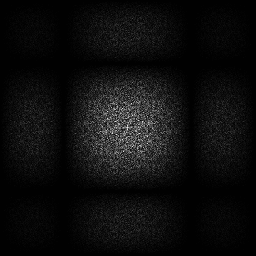
\includegraphics[width=\linewidth]{content/TemporalerAlg/Bilder/Retargeting/Bedeutung Retargeting/SortSerie/seed_debug_3.0_small.png}
       \caption{FT t = 0}
       \label{pic:sortier_t0}
    \end{subfigure}
    \begin{subfigure}[b]{0.2\linewidth}
      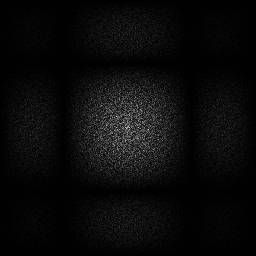
\includegraphics[width=\linewidth]{content/TemporalerAlg/Bilder/Retargeting/Bedeutung Retargeting/SortSerie/seed_debug_4.0_small.png}
      \caption{FT t = 1}
      \label{pic:sortier_t1}
    \end{subfigure}
    \begin{subfigure}[b]{0.2\linewidth}
      
\includegraphics[width=\linewidth]{content/TemporalerAlg/Bilder/Retargeting/Bedeutung Retargeting/SortSerie/seed_debug_5.0_small_screen.png}
      \caption{Ausschnitt t=2}
      \label{pic:sortier_screen_t2}
    \end{subfigure}
    \begin{subfigure}[b]{0.2\linewidth}
        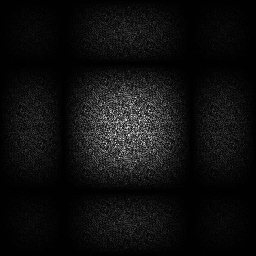
\includegraphics[width=\linewidth]{content/TemporalerAlg/Bilder/Retargeting/Bedeutung Retargeting/SortSerie/seed_debug_5.0_small.png}
        \caption{FT t = 2}
        \label{pic:sortier_t2}
      \end{subfigure}
    
    %%%%%%%%%%%%%%%%%%%%%%%%%%%%%%%%%%%%%%%%%%%%%%%%%%%%%%%%%%%%%%%%%%%%%%%%%%%%%%%%%%%%%%%%%%%%%%%%%%%%%%
    %%%%%%%%%%%%%%%%%%%%%%%%%%%%%%% second row --> sorting block size 2 with retargeting
    %%%%%%%%%%%%%%%%%%%%%%%%%%%%%%%%%%%%%%%%%%%%%%%%%%%%%%%%%%%%%%%%%%%%%%%%%%%%%%%%%%%%%%%%%%%%%%%%%%%%%%

    \begin{subfigure}[b]{0.2\linewidth}
        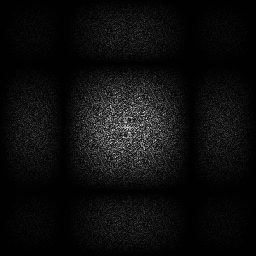
\includegraphics[width=\linewidth]{content/TemporalerAlg/Bilder/Retargeting/Bedeutung Retargeting/RetargetSerie/seed_debug_3.0_small.png}
         \caption{FT t = 0}
         \label{pic:retarget_t0}
    \end{subfigure}
    \begin{subfigure}[b]{0.2\linewidth}
        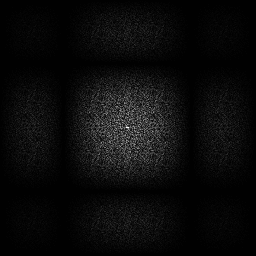
\includegraphics[width=\linewidth]{content/TemporalerAlg/Bilder/Retargeting/Bedeutung Retargeting/RetargetSerie/seed_debug_4.0_small.png}
         \caption{FT t = 1}
         \label{pic:retarget_t1}
    \end{subfigure}
    \begin{subfigure}[b]{0.2\linewidth}
        
\includegraphics[width=\linewidth]{content/TemporalerAlg/Bilder/Retargeting/Bedeutung Retargeting/RetargetSerie/seed_debug_5.0_small_screen.png}
         \caption{Ausschnitt t=2}
         \label{pic:retarget_screen_t2}
    \end{subfigure}
    \begin{subfigure}[b]{0.2\linewidth}
        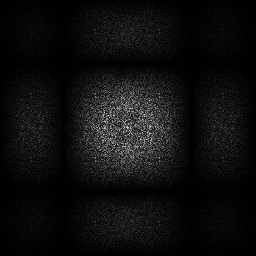
\includegraphics[width=\linewidth]{content/TemporalerAlg/Bilder/Retargeting/Bedeutung Retargeting/RetargetSerie/seed_debug_5.0_small.png}
         \caption{FT t = 2}
         \label{pic:retarget_t2}
    \end{subfigure}
    \caption{Vergleich erste Bilder Sorting(B=2) mit bzw. ohne Retargeting}
    \label{fig:VergleichRetargetSorting}
      
\end{figure}

Die Abbildung \ref{fig:VergleichRetargetSorting} verdeutlicht die Bedeutung des Retargeting 
Schrittes. Sie zeigen dieselben Ausschnitte eines homogenen Szenenausschnitts bzw. die korrespondierende 
Spektra über die ersten drei Bilder. Die erste Reihe mit den Bildern
\begin{itemize}
    \item[a.) - d.)] zeigt auch nach dem dritten Bild keine \nameref{ch:Content1:sec:blue noise} Eigenschaften.
                     Dies liegt an der geringen Blockgröße des Sortierschrittes 
                     (in Abschnitt \ref{subsec:Blockgröße} bereits besprochen). Das Histogramm, Wahrscheinlichkeitsfunktion
                     aller möglichen Pixelwerte, wird mit nur vier Werten approximiert. Diese sehr wage Approximation 
                     hat zur Folge, das die Sortierung einer randomisierten Folge entspricht. Deshalb sind im Bildraum
                     (siehe Bild \ref{pic:sortier_screen_t2}) viele Cluster und die white noise Eigenschaften 
                     (siehe Bild \ref{pic:white noise} im Spektrum zu erkennen.
                     \par 
                    Benutzt man hingegen wie in den Bildern  
    \item[e.) - h.)] zu dem wagen Sortierschritt mit Blockgröße B=2 noch den Retargetingschritt, so akkumulieren sich die 
                    Umverteilungen aus dem Sortierschritt. Trotz der geringen Blockgröße, die nicht reicht, damit nach einem 
                    Bild \nameref{ch:Content1:sec:blue noise} Eigenschaften auftreten und aufgrund der Nutzung einer neuen 
                    Textur (siehe auch Abschnitt \ref{ch:Content1:sec:Quasi-Zufallsfolgen}) innerhalb eines jeden 
                    Bilderstellungsvorgangs wieder verschwimmen würden, können wir bereits im dritten Bild 
                    \ref{ch:Content1:sec:blue noise} Eigenschaften erkennen. Im Bildraum (Bild \ref{pic:retarget_screen_t2})
                    sind die Pixelverbünde verschwunden(=hohe Frequenzen). Dies macht sich im Frequenzraum 
                    (siehe Bild \ref{pic:retarget_t2}) erkenntlich, indem niedere Frequenzen weniger vertreten sind 
                    als bei dem bloßen Sortierschritt (Bild \ref{pic:sortier_t2})
\end{itemize}

An sich ist der Schritt eine bloße Anwendung einer Permutation.\ref{alg:retargetingAlg}

\begin{algorithm}[H]
    \caption{\textbf{Retargeting Schritt}}
    \begin{algorithmic}[1]
        \State //permutation indices from precomputed texture
        \State $retaget_{t}$ = retarget\_texure[calc\_correct\_offset()];
        
        \State $retargetedSeeds(old\_id + retaget_{t}) = incomingSeeds(old\_id);$
        
    \end{algorithmic}
    \label{alg:retargetingAlg}
\end{algorithm}

Wir greifen auf unsere beiden vorberechneten Texturen quasi zufällig (siehe \ref{ch:Content1:sec:Quasi-Zufallsfolgen})
zu. Dabei wird der Permutationswert auf die jeweilige Position des Anfangswertes addiert.
Dabei kann ein jeder Pixel in einem Umfeld (Radius r = 6) permutiert werden (siehe \ref{pic:Permutation}).

\begin{figure}[H]
    \centering
    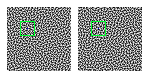
\includegraphics[width=0.5\linewidth]{content/simulatedAnnealing/Bilder/Permutation.png}
    \caption{Permutation}
    \label{pic:Permutation}
\end{figure}

\begin{algorithm}[H]
    \caption{Benutzung unser zwei vorberechneten Texturen: Blue Noise und Retarget}
    \begin{algorithmic}[1]
        \State $bluenoise_{t}$(i,j) = $bluenoise_{0}$(i + $\alpha$t, j + $\beta$t); 
        \State $retarget_{t}$(i,j) = $retarget_{0}$(i + $\alpha$t, j + $\beta$t) + ($\alpha$t, $\beta$t)
    \end{algorithmic}
    \label{alg:Benutzung vorberechneter Texturen}
\end{algorithm}

\newpage
%%%%%%%%%%%%%%%%%%%%%%%%%%%%%%%%%%%%%%%%%%%%%%%%%%%%%%%%%%%%
%%%%%%%%%% Beginning the Sequence of getting to blue noise from white noise
%%%%%%%%%%%%%%%%%%%%%%%%%%%%%%%%%%%%%%%%%%%%%%%%%%%%%%%%%%%%

\label{fig:Retargetbilderstrecke}
\begin{figure}[H]

    \begin{subfigure}{\textwidth}
        \centering 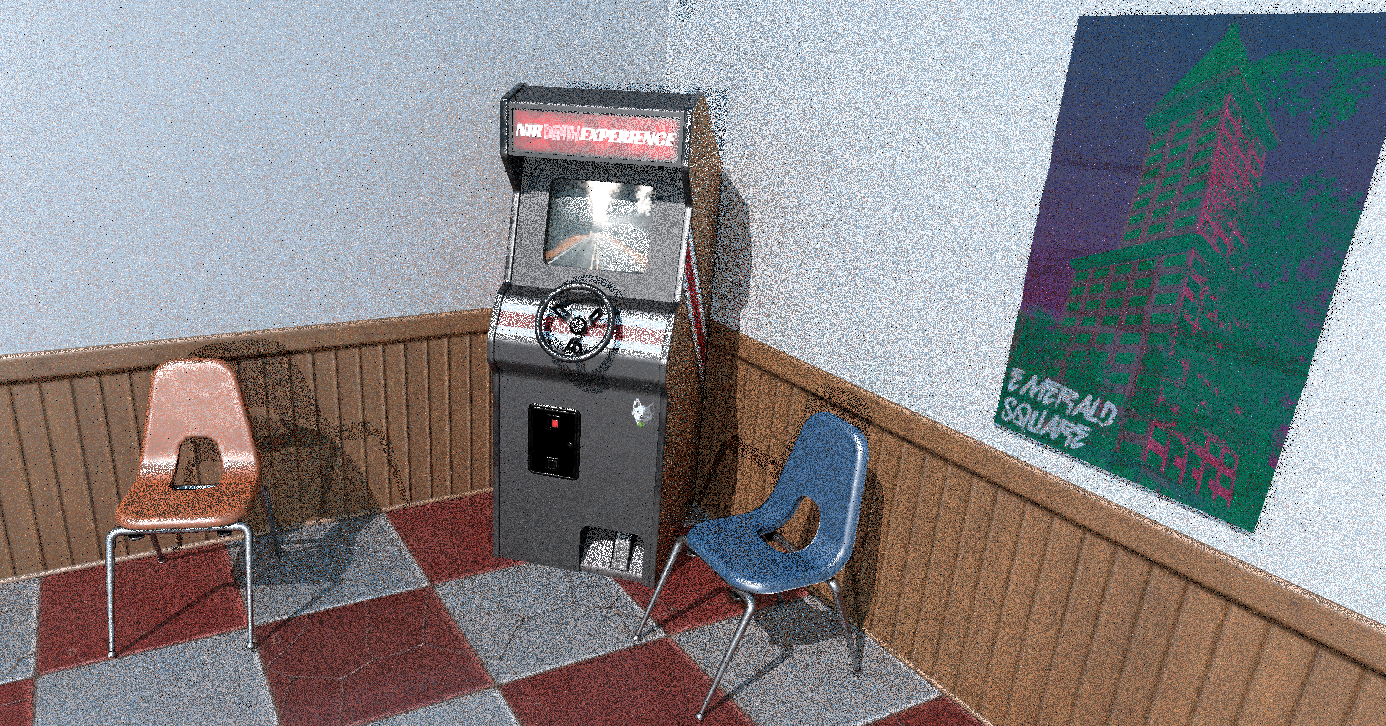
\includegraphics[scale=.25]{content/TemporalerAlg/Bilder/Retargeting/Screenshots/seed_debug_3.0_selection.png}
        \caption{Szene}
        \label{fig:Retargeting_And_Sorting_Szene_t1}
    \end{subfigure}
    \begin{subfigure}{0.5\textwidth}
        \centering 
\includegraphics[width=0.4\linewidth]{content/TemporalerAlg/Bilder/Retargeting/Screenshots/seed_debug_3.0_ausschnitt.png} 
        \caption{Szenenausschnitt}
        \label{fig:Retargeting_And_Sorting_ausschnitt_t1}
    \end{subfigure}
    \begin{subfigure}{0.5\textwidth}
        \centering 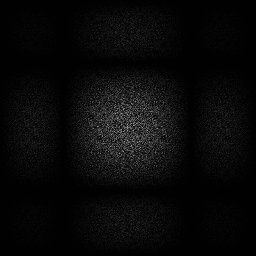
\includegraphics[width=0.4\linewidth]{content/TemporalerAlg/Bilder/Retargeting/Screenshots/Spektren/seed_debug_3.0_ausschnitt.png}
        \caption{Fouriertransformierte des Ausschnitts}
        \label{fig:Retargeting_And_Sorting_Fouriertransformierte_t1}
    \end{subfigure}
        \caption{Zeitpunkt t=1}
        \label{fig:Retargeting_And_Sorting_Verlauf_t1}
\end{figure}

\begin{figure}[H]
    \begin{subfigure}{\textwidth}
        \centering 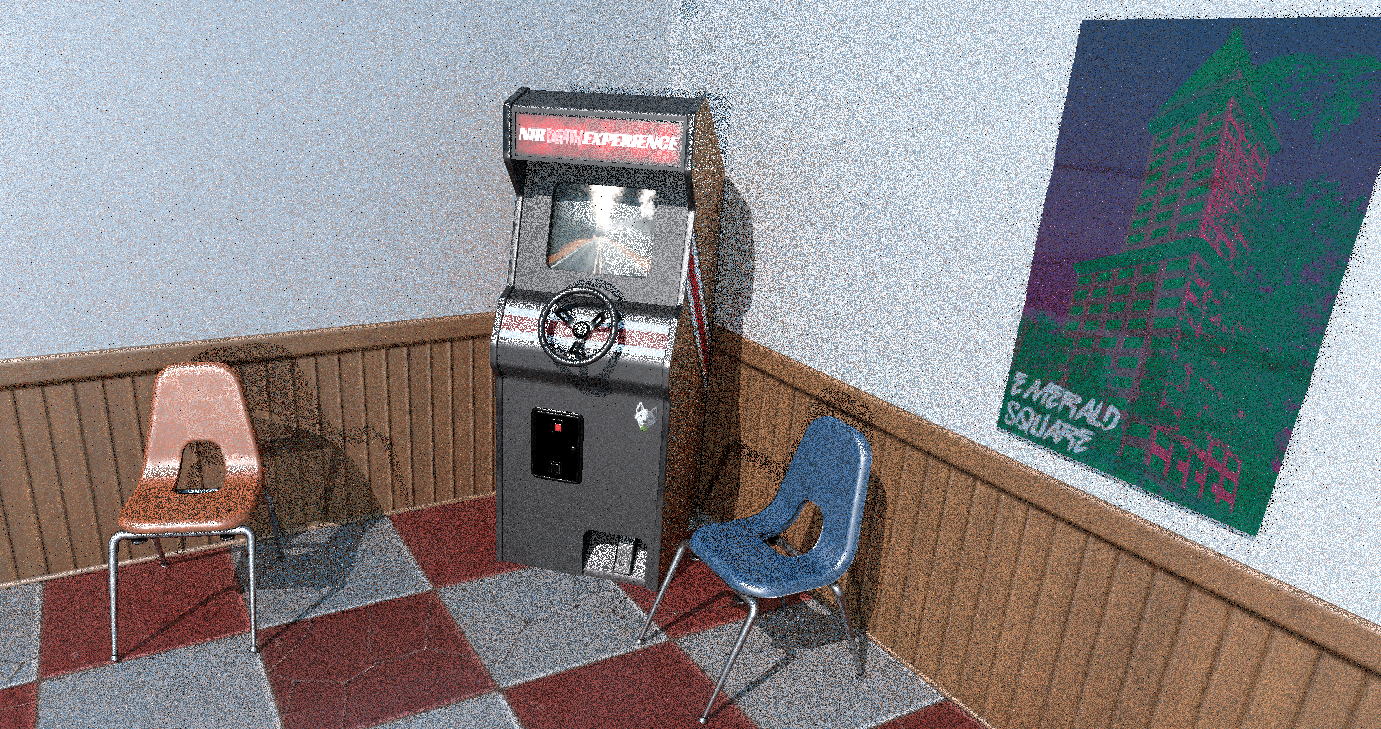
\includegraphics[scale=.25]{content/TemporalerAlg/Bilder/Retargeting/Screenshots/seed_debug_4.0_selection.png}
        \caption{Szene}
        \label{fig:Retargeting_And_Sorting_Szene_t2}
    \end{subfigure}
    \begin{subfigure}{0.5\textwidth}
        \centering
\includegraphics[width=0.4\linewidth]{content/TemporalerAlg/Bilder/Retargeting/Screenshots/seed_debug_4.0_ausschnitt.png} 
        \caption{Szenenausschnitt}
        \label{fig:Retargeting_And_Sorting_ausschnitt_t2}
    \end{subfigure}
    \begin{subfigure}{0.5\textwidth}
        \centering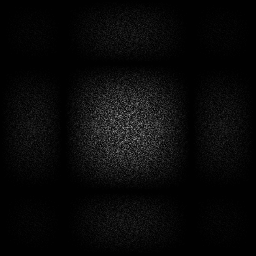
\includegraphics[width=0.4\linewidth]{content/TemporalerAlg/Bilder/Retargeting/Screenshots/Spektren/seed_debug_4.0_ausschnitt.png}
        \caption{Fouriertransformierte des Ausschnitts}
        \label{fig:Retargeting_And_Sorting_Fouriertransformierte_t2}
    \end{subfigure}
        \caption{Zeitpunkt t=2}
        \label{fig:Retargeting_And_Sorting_Verlauf_t2}
\end{figure}

\begin{figure}[H]
    \begin{subfigure}{\textwidth}
        \centering 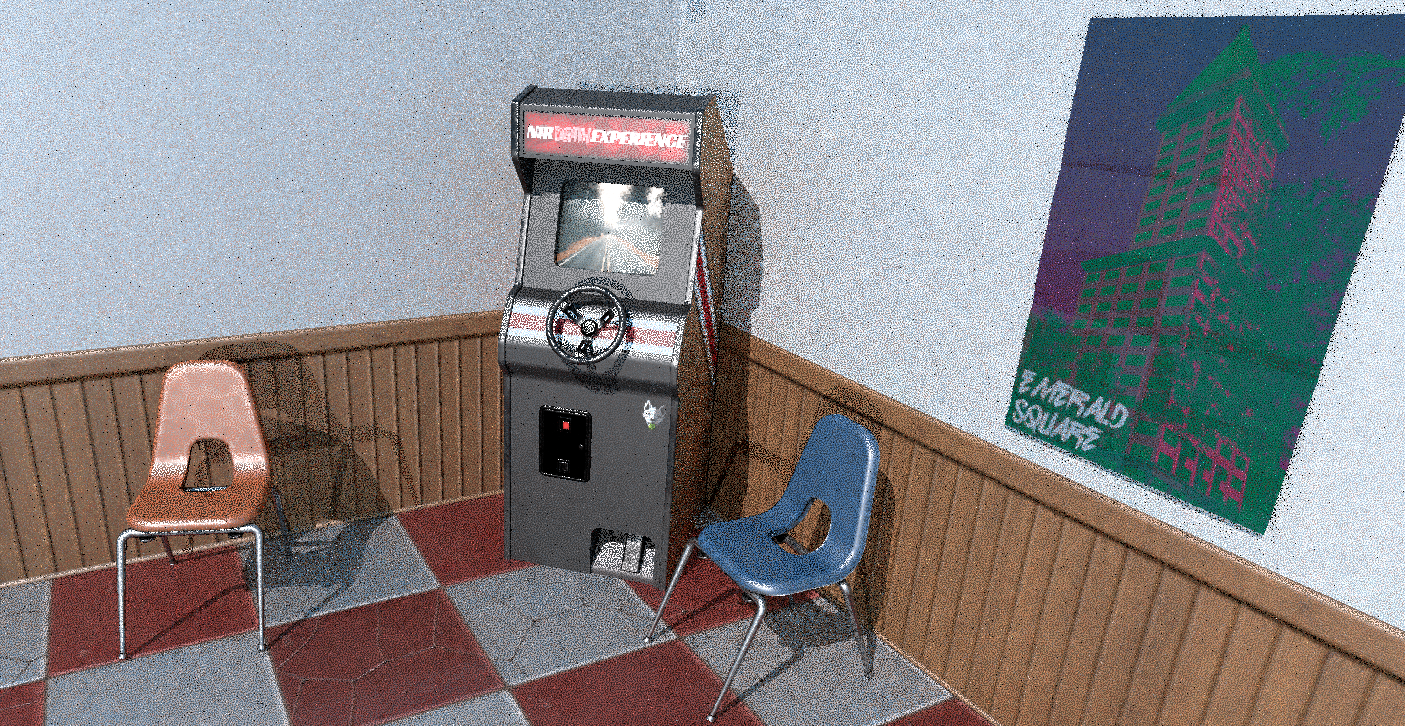
\includegraphics[scale=.25]{content/TemporalerAlg/Bilder/Retargeting/Screenshots/seed_debug_5.0_selection.png}
        \caption{Szene}
        \label{fig:Retargeting_And_Sorting_Szene_t3}
    \end{subfigure}
    \begin{subfigure}{0.5\textwidth}
        \centering
\includegraphics[width=0.4\linewidth]{content/TemporalerAlg/Bilder/Retargeting/Screenshots/seed_debug_5.0_ausschnitt.png} 
        \caption{Szenenausschnitt}
        \label{fig:Retargeting_And_Sorting_ausschnitt_t3}
    \end{subfigure}
    \begin{subfigure}{0.5\textwidth}
        \centering
\includegraphics[width=0.4\linewidth]{content/TemporalerAlg/Bilder/Retargeting/Screenshots/Spektren/seed_debug_5.0_ausschnitt.png}
        \caption{Fouriertransformierte des Ausschnitts}
        \label{fig:Retargeting_And_Sorting_Fouriertransformierte_t3}
    \end{subfigure}
        \caption{Zeitpunkt t=3}
        \label{fig:Retargeting_And_Sorting_Verlauf_t3}
\end{figure}

\begin{figure}[H]
    \begin{subfigure}{\textwidth}  
        \centering 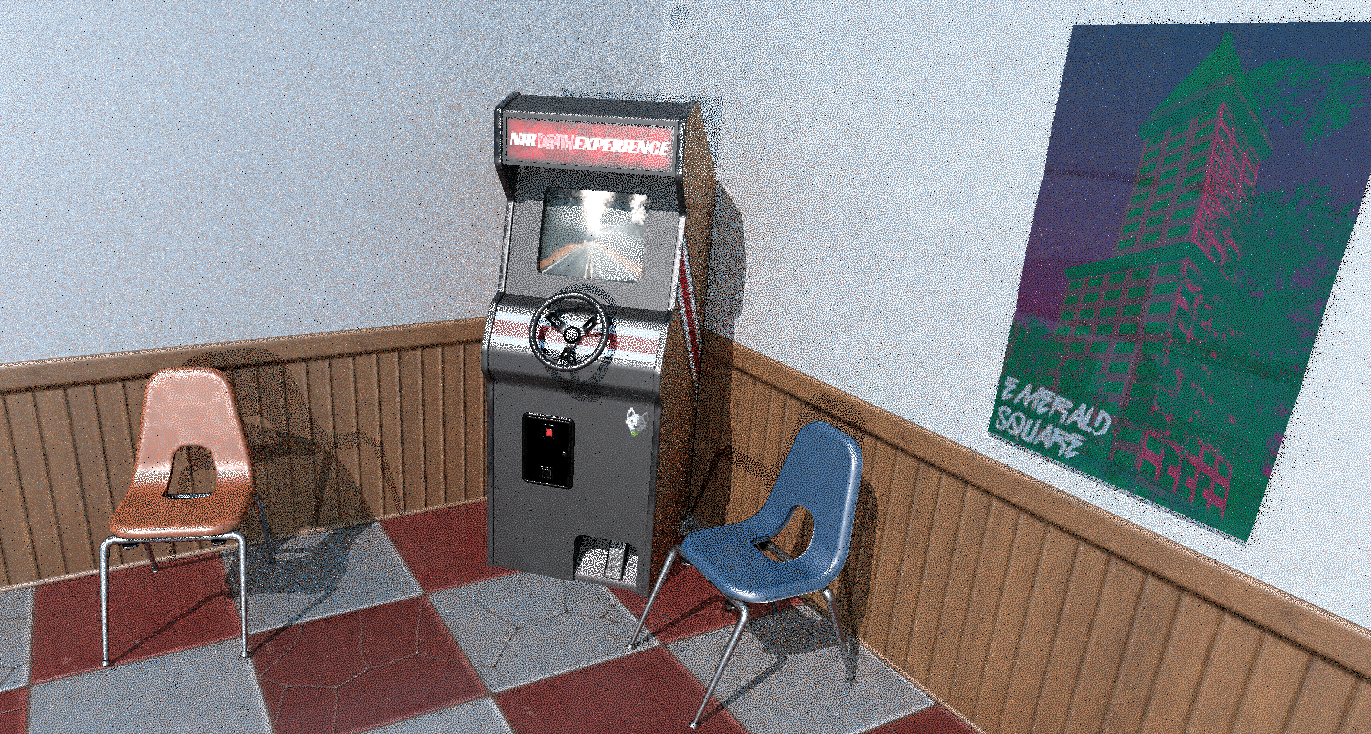
\includegraphics[scale=.25]{content/TemporalerAlg/Bilder/Retargeting/Screenshots/seed_debug_6.0_selection.png}
        \caption{Szene}
        \label{fig:Retargeting_And_Sorting_Szene_t4}
    \end{subfigure}
    \begin{subfigure}{0.5\textwidth}
        \centering
\includegraphics[width=0.4\linewidth]{content/TemporalerAlg/Bilder/Retargeting/Screenshots/seed_debug_6.0_ausschnitt.png} 
        \caption{Szenenausschnitt}
        \label{fig:Retargeting_And_Sorting_ausschnitt_t4}
    \end{subfigure}
    \begin{subfigure}{0.5\textwidth}
        \centering
\includegraphics[width=0.4\linewidth]{content/TemporalerAlg/Bilder/Retargeting/Screenshots/Spektren/seed_debug_6.0_ausschnitt.png}
        \caption{Fouriertransformierte des Ausschnitts}
        \label{fig:Retargeting_And_Sorting_Fouriertransformierte_t4}
    \end{subfigure}
        \caption{Zeitpunkt t=4}
        \label{fig:Retargeting_And_Sorting_Verlauf_t4}
\end{figure}

\begin{figure}[H]
    \begin{subfigure}{\textwidth}   
        \centering 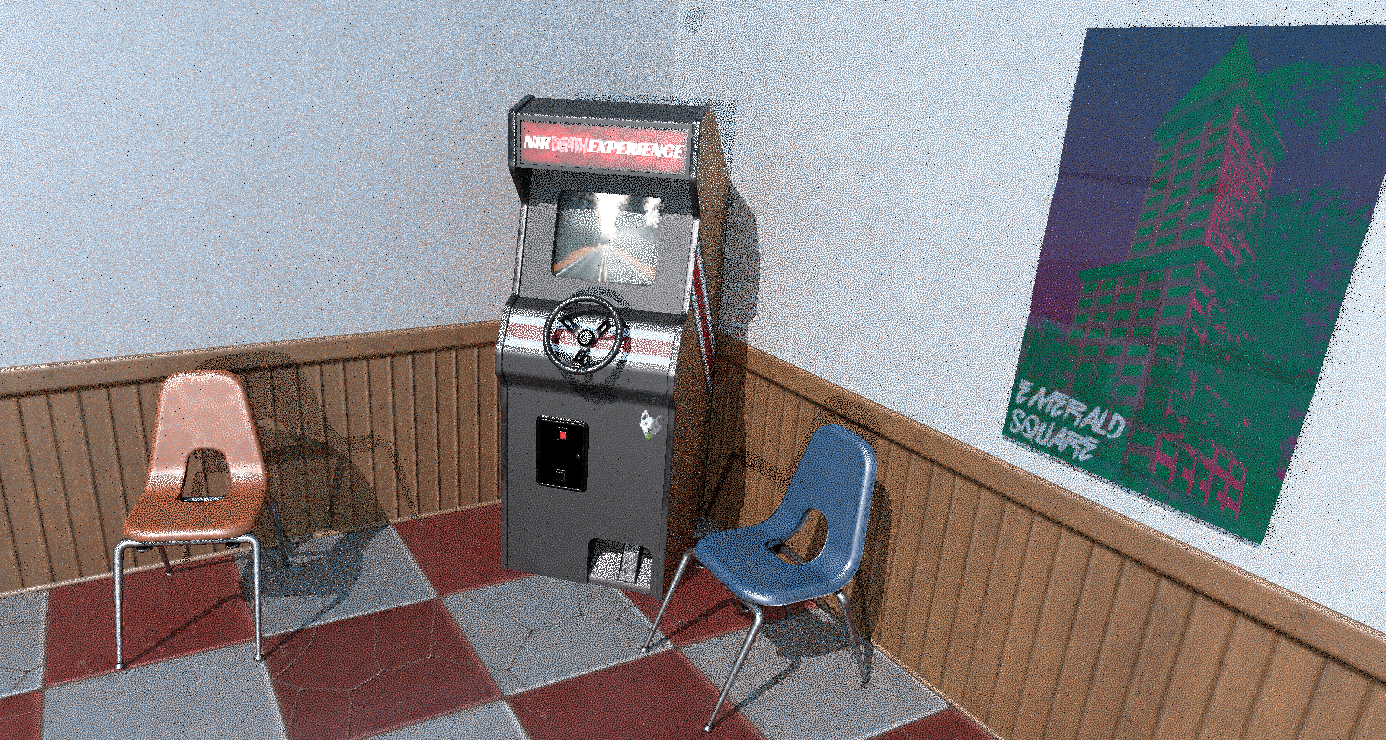
\includegraphics[scale=.25]{content/TemporalerAlg/Bilder/Retargeting/Screenshots/seed_debug_7.0_selection.png}
        \caption{Szene}
        \label{fig:Retargeting_And_Sorting_Szene_t5}
    \end{subfigure}
    \begin{subfigure}{0.5\textwidth}
        \centering
\includegraphics[width=0.4\linewidth]{content/TemporalerAlg/Bilder/Retargeting/Screenshots/seed_debug_7.0_ausschnitt.png} 
        \caption{Szenenausschnitt}
        \label{fig:Retargeting_And_Sorting_ausschnitt_t5}
    \end{subfigure}
    \begin{subfigure}{0.5\textwidth}
        \centering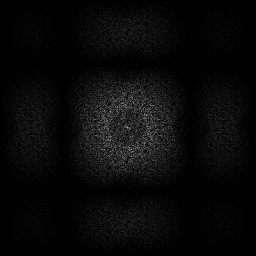
\includegraphics[width=0.4\linewidth]{content/TemporalerAlg/Bilder/Retargeting/Screenshots/Spektren/seed_debug_7.0_ausschnitt.png}
        \caption{Fouriertransformierte des Ausschnitts}
        \label{fig:Retargeting_And_Sorting_Fouriertransformierte_t5}
    \end{subfigure}
        \caption{Zeitpunkt t=5}
        \label{fig:Retargeting_And_Sorting_Verlauf_t5}
\end{figure}

\begin{figure}[H]
    \begin{subfigure}{\textwidth}   
        \centering 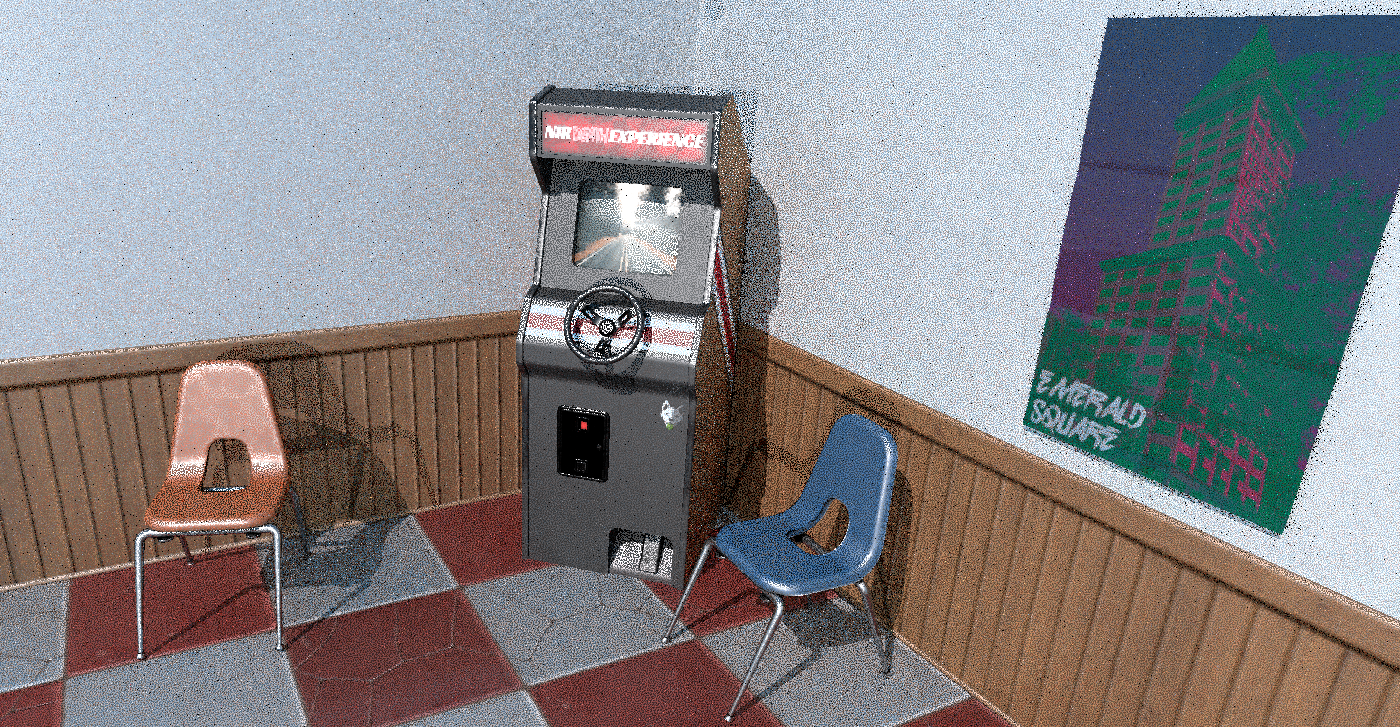
\includegraphics[scale=.25]{content/TemporalerAlg/Bilder/Retargeting/Screenshots/seed_debug_8.0_selection.png}
        \caption{Szene}
        \label{fig:Retargeting_And_Sorting_Szene_t6}
    \end{subfigure}
    \begin{subfigure}{0.5\textwidth}
        \centering
\includegraphics[width=0.4\linewidth]{content/TemporalerAlg/Bilder/Retargeting/Screenshots/seed_debug_8.0_ausschnitt.png} 
        \caption{Szenenausschnitt}
        \label{fig:Retargeting_And_Sorting_ausschnitt_t6}
    \end{subfigure}
    \begin{subfigure}{0.5\textwidth}
        \centering
\includegraphics[width=0.4\linewidth]{content/TemporalerAlg/Bilder/Retargeting/Screenshots/Spektren/seed_debug_8.0_ausschnitt.png}
        \caption{Fouriertransformierte des Ausschnitts}
        \label{fig:Retargeting_And_Sorting_Fouriertransformierte_t6}
    \end{subfigure}
        \caption{Zeitpunkt t=6}
        \label{fig:Retargeting_And_Sorting_Verlauf_t6}
\end{figure}

\begin{figure}[H]
    \begin{subfigure}{\textwidth}   
        \centering 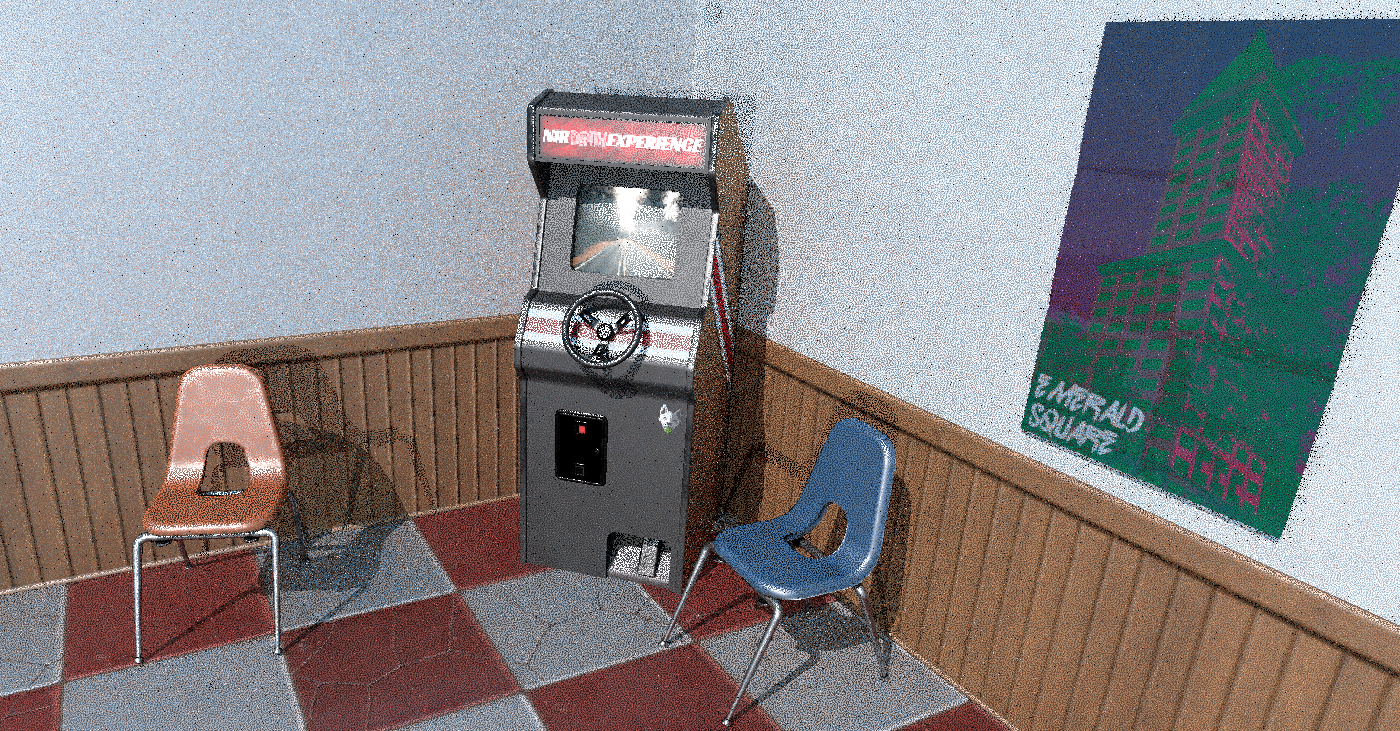
\includegraphics[scale=.25]{content/TemporalerAlg/Bilder/Retargeting/Screenshots/seed_debug_9.0_selection.png}
        \caption{Szene}
        \label{fig:Retargeting_And_Sorting_Szene_t7}
    \end{subfigure}
    \begin{subfigure}{0.5\textwidth}
        \centering
\includegraphics[width=0.4\linewidth]{content/TemporalerAlg/Bilder/Retargeting/Screenshots/seed_debug_9.0_ausschnitt.png} 
        \caption{Szenenausschnitt}
        \label{fig:Retargeting_And_Sorting_ausschnitt_t7}
    \end{subfigure}
    \begin{subfigure}{0.5\textwidth}
        \centering
\includegraphics[width=0.4\linewidth]{content/TemporalerAlg/Bilder/Retargeting/Screenshots/Spektren/seed_debug_9.0_ausschnitt.png}
        \caption{Fouriertransformierte des Ausschnitts}
        \label{fig:Retargeting_And_Sorting_Fouriertransformierte_t7}
    \end{subfigure}
        \caption{Zeitpunkt t=7}
        \label{fig:Retargeting_And_Sorting_Verlauf_t7}
\end{figure}

Im dritten Bild der Reihe \ref{fig:Retargeting_And_Sorting_Verlauf_t3} können wir eine erste 
\ref{ch:Content1:sec:blue noise} Fehlerverteilung im Bildraum erkennen. Im Gegensatz zum 
reinen \nameref{ch:Content2:sec:Sorting} ohne dem Retargetingschritt haben wir hier in den 
Bildern danach \ref{fig:Retargeting_And_Sorting_Verlauf_t4} - \ref{fig:Retargeting_And_Sorting_Verlauf_t7}
keine so starke Abschwächung der Verteilung zwischen den Bildern sondern eine Akkumulation.

\begin{figure}[H]
    \begin{subfigure}{0.5\textwidth}
        \centering
\includegraphics[width=0.5\linewidth]{content/TemporalerAlg/Bilder/Sorting/Screenshots/Spektren/seed_debug_9.0_ausschnitt.png} 
        \caption{FFT reines Sorting}
        \label{fig:VergleichSorting}
    \end{subfigure}
    \begin{subfigure}{0.5\textwidth}
        \centering
\includegraphics[width=0.5\linewidth]{content/TemporalerAlg/Bilder/Retargeting/Screenshots/Spektren/seed_debug_9.0_ausschnitt.png}
        \caption{FFT Sorting + Retargeting}
        \label{fig:VergleichRetargeting}
    \end{subfigure}
        \caption{Vergleich des siebten Bildes vom reinen Sorting und zusätzlichem Retargeting}
        \label{fig:VergleichBild7}
\end{figure}

Das siebte Bild \ref{fig:VergleichBild7} nach Beginn steht beispielhaft für die Akkumulation des Retargeting Schrittes bzw. 
dem Verwischen der \ref{ch:Content1:sec:blue noise} Verteilung bei bloßem Sorting aufgrund ständig 
wechselnder blue noise Textur.